% The FYP template is designed according to NTU SCSE FYP guidelines on https://www3.ntu.edu.sg/scse/fyp/UsefulInfo/Report%20Guide.pdf.

% Credit
% Original version by Vincent Ribli
% https://www.overleaf.com/latex/templates/ntu-scse-fyp-template/kwdtcbqmjctk

% Revised by Prof Loy Chen Change
% 23 Aug 2024 - Replace SCSE with CCDS


\documentclass[pdftex, 12pt, a4paper]{report}
\usepackage{newtxtext, newtxmath}
\usepackage[top=3cm, bottom=3cm, left=3.5cm, right=3cm]{geometry}
\usepackage[hidelinks]{hyperref}
\usepackage[pdftex]{graphicx}
\usepackage{booktabs}
\usepackage{setspace}
\usepackage{titlesec}
\usepackage{tocloft}
\usepackage{parskip}
\usepackage{amsmath}
\usepackage{amsfonts}
\usepackage[sorting=none]{biblatex}

% Additional packages
\usepackage{listings}
\usepackage{tabularx}
\usepackage{xcolor}
\usepackage{multirow}
\usepackage{float}
\usepackage{makecell}

% Code listing style
\definecolor{codegreen}{rgb}{0,0.6,0}
\definecolor{codegray}{rgb}{0.5,0.5,0.5}
\definecolor{codepurple}{rgb}{0.58,0,0.82}
\definecolor{backcolour}{rgb}{0.95,0.95,0.92}
\lstdefinestyle{mystyle}{
    backgroundcolor=\color{backcolour},
    commentstyle=\color{codegreen},
    keywordstyle=\color{magenta},
    numberstyle=\tiny\color{codegray},
    stringstyle=\color{codepurple},
    basicstyle=\ttfamily\footnotesize,
    breakatwhitespace=false,
    breaklines=true,
    captionpos=b,
    keepspaces=true,
    numbers=left,
    numbersep=5pt,
    showspaces=false,
    showstringspaces=false,
    showtabs=false,
    tabsize=2
}
\lstset{style=mystyle}
\lstset{breaklines=true}

\addbibresource{bib.bib}
\setstretch{1.5}
\setlength{\cftfigindent}{0pt}
\setlength{\cfttabindent}{0pt}
\renewcommand{\cftdotsep}{1}


% change the following
\title{\uppercase{Advancing Spatial and Embodied Intelligence in Multimodal Foundation Models}}
\newcommand\fypcode{CCDS4016}
\author{Qian Jianheng Oscar}
\date{2026}
\newcommand\degree{Bachelor of Science in Data Science and Artificial Intelligence}
\newcommand\supervisor{Prof. Ziwei Liu}

\begin{document}
\makeatletter
\begin{titlepage}
\begin{center}


\includegraphics[width=0.5\textwidth]{fig/ntu_logo.png}
\\[0.5cm]
\uppercase{\textbf{\large{Nanyang Technological University}}}
\\[4cm]

\uppercase{\textbf{\fypcode \\[0.3cm]\@title}}

\vfill

Submitted in Partial Fulfilment of the Requirements\\
for the Degree of \degree\\
of the Nanyang Technological University
\\[0.8cm]
by
\\[0.8cm]

\@author
\\[2cm]
Supervisor: Prof. Ziwei Liu
\end{center}

College of Computing and Data Science\\
\@date
\end{titlepage}
\makeatother


\setcounter{page}{1}
\pagenumbering{roman}

\chapter*{Abstract}
\addcontentsline{toc}{chapter}{Abstract}

Spatial intelligence---the ability to perceive, reason about, and interact with the three-dimensional physical world---remains one of the most significant gaps in modern multimodal AI. This report documents research conducted at SenseTime Research from October 2025 to March 2026, tracing a narrative from diagnosing the spatial reasoning deficiencies of frontier models, through data-driven efforts to close that gap, to the open question of whether static benchmark gains translate into interactive embodied competence. The work spans contributions to two publications~\cite{cai2025holisticevaluationmultimodalllms, cai2025scalingspatialintelligencemultimodal} and the independent development of a unified embodied evaluation toolkit, together forming a coherent investigation into what it takes to make multimodal models spatially intelligent.

\chapter*{Acknowledgments}
\addcontentsline{toc}{chapter}{Acknowledgments}

I would like to express my gratitude to Dr. Cai Zhongang and the SenseTime Research team for their guidance and support during this research attachment. Their expertise in spatial intelligence and multimodal evaluation shaped the direction of this work and provided invaluable feedback throughout.

\vspace{1em}

\textbf{Statement of Contributions.} To maintain academic integrity and clearly attribute credit, this section distinguishes between team-level work and my individual contributions.

Within the EASI project~\cite{cai2025holisticevaluationmultimodalllms, cai2025scalingspatialintelligencemultimodal}, I was responsible for evaluation infrastructure. This encompassed integrating nine spatial benchmarks (VSI-Bench variants, ViewSpatial, SITE, SparBench, MMSI-Video, OSI-Bench, 3DSR-Bench, MindCube-Tiny) and two models (Cambrian-S, Bagel) into lmms-eval, fixing inference bugs in Qwen3-VL, InternVL, LLaVA-OV, and Cambrian-S, and running evaluations across models and benchmarks. This infrastructure was used to produce the results in both publications.

The EASI spatial intelligence taxonomy, paper writing and narrative design, SenseNova-SI-8M dataset curation and synthesis, model training and SFT experiments, data scaling analysis, emergent capability analysis, overfitting and shortcut studies, spatial chain-of-thought experiments, and qualitative failure analysis were all conducted by other team members.

The EASI embodied evaluation library is entirely my own design and implementation. This includes the full software architecture, all ten benchmark integrations across five simulators, the parallel evaluation pipeline with vLLM support and the 540+ test suite.


\pagebreak
\addcontentsline{toc}{chapter}{Contents}
\tableofcontents

\pagebreak
\addcontentsline{toc}{chapter}{List of Tables}
\listoftables

\pagebreak
\addcontentsline{toc}{chapter}{List of Figures}
\listoffigures

\cleardoublepage
\pagenumbering{arabic}

\chapter{Introduction}
\label{sec:introduction}

In early 2025, a curious pattern emerged across the multimodal AI landscape. Models like GPT-4o and Gemini-1.5 could describe images in exquisite detail, answer complex questions about charts and documents, and even reason about abstract visual puzzles, yet they struggled with questions that a child could answer intuitively. \textit{``Which object is closer to the camera?''} \textit{``If you turned around, what would you see?''} \textit{``How far apart are the chair and the desk?''} These are not exotic tasks; they are the bread and butter of how humans navigate the physical world.

This observation motivated the research that this report documents. The central thesis is simple but important. Spatial intelligence is both critically important and underserved by current evaluation and training paradigms. The work proceeds in three phases. First, we ask, \textit{how bad is the problem, really?} To answer this rigorously requires a holistic evaluation framework that goes beyond individual benchmarks. Second, armed with a precise diagnosis of what models get wrong, we ask, \textit{can we fix it through data?} Specifically, can curating and scaling spatial training data systematically improve these capabilities? Third, and most ambitiously, \textit{does any of this matter for agents that must act in the real world?} Static benchmarks test perception and reasoning in isolation, but embodied agents must also plan, execute, and recover from failure in interactive 3D environments.

Three questions---diagnosis, treatment, and validation---structure the report.

\chapter{Background and Related Work}
\label{sec:background}

\section{What Is Spatial Intelligence?}

Spatial intelligence is not a single capability but a family of related skills. Following the taxonomy proposed in~\cite{cai2025holisticevaluationmultimodalllms}, we decompose it into six fundamental dimensions.

\textbf{Metric Measurement (MM)} involves understanding physical scale such as estimating distances between objects, gauging the size of a room, or judging whether a sofa would fit through a doorway. \textbf{Spatial Relations (SR)} captures the ability to reason about relative positions of multiple objects within a 3D coordinate system. \textbf{Mental Reconstruction (MR)} requires inferring a detailed spatial representation of an object from limited 2D views. \textbf{Perspective-Taking (PT)} is perhaps the most demanding as it requires reasoning about how a scene appears from different viewpoints, establishing correspondences across views, inferring camera motion, and mentally simulating viewpoint shifts. \textbf{Deformation and Assembly (DA)} addresses scenarios where objects change shape or must be combined, for example understanding how a flat sheet folds into a box, tracing the steps of tying a knot, or figuring out how separate components fit together into a whole. Finally, \textbf{Comprehensive Reasoning (CR)} involves coordinating multiple spatial capabilities across multi-step reasoning chains.

This taxonomy proved essential for the work that followed. Without it, evaluation results would be a soup of numbers from disparate benchmarks; with it, we could precisely identify which spatial capabilities are strong, which are weak, and where targeted intervention is most needed.

\section{The Benchmark Landscape}

A growing ecosystem of benchmarks has emerged to test these capabilities, each covering a different slice of the space. VSI-Bench~\cite{yang2025thinkingspacemultimodallarge} evaluates video-based spatial reasoning (object counting, distance estimation, route planning) using egocentric indoor video. MMSI~\cite{yang2025mmsibenchbenchmarkmultiimagespatial} tests multi-image spatial understanding, focusing on positional relationships between cameras, objects, and regions. MindCube~\cite{yin2025spatialmentalmodelinglimited} probes whether models can infer what lies beyond the visible frame, such as filling in unobserved regions, adopting novel viewpoints, and predicting the outcome of hypothetical movements given only a few reference images. ViewSpatial~\cite{li2025viewspatialbenchevaluatingmultiperspectivespatial} probes view-dependent spatial reasoning. SITE~\cite{wang2025sitespatialintelligencethorough} provides a multi-choice VQA benchmark spanning single-image, multi-image, and video modalities, testing spatial visualization, orientation, and dynamic scene reasoning at both figural and environmental scales. OmniSpatial~\cite{jia2026omnispatialcomprehensivespatialreasoning} spans dynamic reasoning, spatial interaction, complex logic, and perspective-taking.

The fragmentation is the problem. Each benchmark uses its own evaluation protocol, prompt format, and metric. A model might score well on VSI-Bench's object counting but poorly on its route planning; it might handle MMSI's camera-camera correspondences but fail on object-object ones. Without a unified framework, comparing models across the full breadth of spatial capabilities is impractical.

\section{Approaches to Improving Spatial Reasoning}

Efforts to close the spatial intelligence gap follow two broad strategies. Architecture-based approaches incorporate 3D-aware encoders. Spatial-MLLM~\cite{wu2025spatialmllmboostingmllmcapabilities} pairs a standard 2D encoder with a visual geometry foundation model to extract 3D structural features from 2D inputs, VLM-3R~\cite{fan2025vlm3rvisionlanguagemodelsaugmented} derives implicit 3D tokens from monocular video via a geometry encoder, 3DThinker~\cite{chen2026think3dgeometricimagination} teaches VLMs to generate 3D latent representations during reasoning by aligning them with a 3D foundation model, then refining through outcome-based reinforcement learning. Data-centric approaches instead curate spatial training data and apply supervised fine-tuning (SFT) or reinforcement learning (RL). SpatialVLM~\cite{chen2024spatialvlmendowingvisionlanguagemodels} pioneered this direction with 2 billion synthetic spatial QA samples. Subsequent work includes SpatialLadder (26K samples with progressive training)~\cite{li2025spatialladderprogressivetrainingspatial}, VST (4.1M SFT + 135K RL samples)~\cite{yang2025visualspatialtuning}, and Cambrian-S (590K spatial video samples with four-stage training)~\cite{yang2025cambriansspatialsupersensingvideo}.

The data-centric approach is appealing because it does not require modifying model architectures, meaning any foundation model can potentially benefit. But the question of \textit{which} data, \textit{how much}, and \textit{organized how} remained open.

\section{From Static Benchmarks to Embodied Agents}

Static benchmarks, however comprehensive, test spatial intelligence in a fundamentally passive mode where the model receives images or video frames and answers questions. But spatial intelligence exists for action. Humans develop spatial reasoning not as an academic exercise but because it enables us to navigate rooms, manipulate objects, and coordinate with others in shared physical spaces.

Embodied AI benchmarks close this gap by placing agents in simulated 3D environments where they must perceive, reason, plan, and act. EmbodiedBench~\cite{yang2025embodiedbenchcomprehensivebenchmarkingmultimodal} provides a multi-domain evaluation spanning household tasks, navigation, habitat exploration, and robotic manipulation. HAZARD~\cite{zhou2024hazardchallengeembodieddecision} places agents in emergency scenarios (fire, flood, wind) where the goal is not explicitly specified as a point-to-point instruction but must be inferred from context, testing whether agents can reason about implicit objectives like prioritising and evacuating valuable objects from danger. VLN-CE~\cite{krantz2020navgraphvisionandlanguagenavigationcontinuous} requires translating natural language navigation instructions into continuous movement through realistic indoor environments. ManipulaTHOR~\cite{ehsani2021manipulathorframeworkvisualobject} tests arm-based point navigation requiring precise spatial positioning.

These benchmarks are expensive to run (each requiring its own simulator, conda environment, and GPU resources) and have historically been evaluated in isolation. No unified framework existed for running them all under a common protocol.

\chapter{Diagnosing the Problem: Holistic Evaluation of Spatial Intelligence}
\label{sec:diagnosis}

\section{Building the Evaluation Infrastructure}

The first phase of work addressed a practical prerequisite. Before we could holistically evaluate spatial intelligence, we needed the benchmarks to actually work within a unified evaluation framework. The lmms-eval framework~\cite{Zhang_2025} provided the foundation, but most spatial benchmarks had not yet been integrated.

I integrated nine spatial benchmarks into lmms-eval, including VSI-Bench in its debiased and pruned variants (removing annotation shortcuts that could inflate scores), a multi-image variant of VSI-Bench (critical for models that handle frame sequences differently from single images), ViewSpatial, SITE, SparBench, MMSI-Video, OSI-Bench, 3DSR-Bench, and a bugfix for MindCube-Tiny. Each integration required implementing the benchmark's specific evaluation protocol (prompt templates, answer extraction, metric computation) and validating results against published baselines.

Alongside the benchmarks, I integrated two models that would serve as important baselines, namely Cambrian-S, a spatial intelligence model family trained on 590K spatial video samples, and Bagel, a unified understanding-and-generation model. I also fixed several inference bugs that surfaced during large-scale evaluation. Qwen3-VL was incorrectly sampling video frames due to an nframes bug, InternVL had an image token formatting issue in interleaved multi-image mode, and various issues appeared in LLaVA-OV-1.5, InternVL3, and Cambrian-S when processing certain benchmark formats. These fixes were essential because without them, the evaluation results for these models would have been unreliable.

\section{The EASI Evaluation Framework}

With the infrastructure in place, the team conducted a comprehensive evaluation across eight key benchmarks~\cite{cai2025holisticevaluationmultimodalllms}. The study, titled \textit{``Holistic Evaluation of Multimodal LLMs on Spatial Intelligence''} (EASI), tested the leading proprietary models (GPT-5, Gemini-2.5-Pro, Grok-4, Seed-1.6) and open-source models (Qwen2.5-VL, InternVL3, and others).

The EASI framework's core contribution is a unified evaluation protocol that maps every benchmark subtask onto the six-capability taxonomy, enabling apples-to-apples comparison across models and capabilities. A standardized zero-shot chain-of-thought prompt is applied uniformly, and results are reported both per-benchmark and aggregated by capability.

\section{What the Evaluation Revealed}

Table~\ref{tab:main_results} presents the main results across eight spatial intelligence benchmarks. Four of these benchmarks (VSI-Bench, SITE, MMSI, and MindCube-Tiny) were evaluated using the integrations I built in lmms-eval, while OmniSpatial, STARE, CoreCognition, and SpatialViz were integrated by other team members.

\begin{table}[htbp]
\centering
\caption{Evaluation on eight spatial intelligence benchmarks (Official Protocol), adapted from~\cite{cai2025holisticevaluationmultimodalllms}. MindCube* denotes MindCube-Tiny. Proprietary model versions: Seed-1.6 (2025-06-15), Gemini-2.5-Pro (2025-06), Grok-4 (2025-07-09), GPT-5 family (2025-08-07).}
\label{tab:main_results}
\renewcommand{\arraystretch}{1.1}
\footnotesize
\setlength{\tabcolsep}{4pt}
\begin{tabular}{lcccccccc}
\toprule
\textbf{Model} & \textbf{VSI} & \textbf{SITE} & \textbf{MMSI} & \textbf{Omni.} & \textbf{MindC.*} & \textbf{STARE} & \textbf{CoreC.} & \textbf{Spat.Viz} \\
\textit{Metric} & \textit{MRA,Acc} & \textit{CAA} & \textit{Acc} & \textit{Acc} & \textit{Acc} & \textit{Acc,F1} & \textit{Acc} & \textit{Acc} \\
\midrule
Random Choice & 34.0 & 0.0 & 25.0 & 25.0 & 32.4 & 34.8 & 33.9 & 25.1 \\
\midrule
\multicolumn{9}{l}{\textit{Proprietary}} \\
Seed-1.6 & 49.9 & 54.6 & 38.3 & 49.3 & 48.8 & 46.1 & 77.2 & 34.6 \\
Gemini-2.5-Pro & 53.6 & 57.1 & 38.0 & 55.4 & 57.6 & 49.1 & 76.7 & 42.7 \\
Grok-4 & 47.9 & 47.0 & 37.8 & 46.8 & 63.6 & 26.9 & 79.3 & 19.4 \\
GPT-5-nano & 43.2 & 35.8 & 28.9 & 47.8 & 41.5 & 46.1 & 67.9 & 35.6 \\
GPT-5-mini & 48.7 & 52.5 & 34.1 & 55.5 & 56.7 & 52.5 & 77.8 & 44.7 \\
GPT-5 & \textbf{55.0} & \textbf{61.9} & \textbf{41.8} & \textbf{59.9} & 56.3 & \textbf{54.6} & \textbf{84.4} & \textbf{51.3} \\
\midrule
\multicolumn{9}{l}{\textit{Open-source}} \\
Qwen2.5-VL-3B & 27.0 & 33.1 & 28.6 & 42.5 & 37.6 & 37.8 & 60.2 & 21.9 \\
Qwen2.5-VL-7B & 32.3 & 37.6 & 26.8 & 39.1 & 36.1 & 35.0 & 62.2 & 26.8 \\
Qwen2.5-VL-72B & 35.8 & 47.4 & 32.5 & 47.8 & 42.4 & 38.4 & 69.2 & 32.5 \\
InternVL3-8B & 42.1 & 41.2 & 28.0 & 46.3 & 41.5 & 41.4 & 60.9 & 30.0 \\
InternVL3-78B & 47.6 & 52.7 & 30.5 & 51.0 & 49.5 & 42.0 & 71.2 & 31.1 \\
InternVL3.5-8B & 56.1 & 43.8 & 27.3 & 46.7 & 42.5 & 40.2 & 66.4 & 24.0 \\
Qwen3-8B & 57.9 & 45.8 & 31.1 & 45.7 & 29.4 & 39.8 & 69.7 & 17.5 \\
\midrule
\textbf{Human} & \textbf{79.2} & \textbf{67.5} & \textbf{97.2} & \textbf{92.6} & \textbf{94.6} & \textbf{96.5} & \textbf{87.0} & \textbf{82.5} \\
$\Delta$ (best $-$ human) & $-$21.3 & $-$5.6 & $-$55.4 & $-$32.7 & $-$31.0 & $-$42.1 & $-$2.6 & $-$31.2 \\
\bottomrule
\end{tabular}
\end{table}

The results painted a stark picture. GPT-5, the most powerful model tested, set a new state of the art, yet the human-model gap remained enormous on most benchmarks. Consider the MMSI column, which I integrated into lmms-eval, humans score 97.2\% while GPT-5 manages just 41.8\%, a gap of over 55 points. On MindCube-Tiny (another benchmark I integrated, with its evaluation bugs fixed), human performance of 94.6\% dwarfs GPT-5's 56.3\%. Even SITE, where the gap appears smallest at 5.6 points, benefits from a relatively low human baseline of 67.5\%; the model's 61.9\% is impressive but deceptive without context.

More revealing than the absolute gaps were the patterns across capabilities. Perspective-taking (PT) and metric measurement (MM) emerged as the weakest dimensions across all models. Drilling into the per-subtask breakdowns that I helped produce by running evaluations across models, the picture sharpened further. On MMSI's camera-to-camera perspective-taking questions, the best model (GPT-5) scored 41.9\% against a human baseline of 95.7\%, a gap of over 53 points. On MindCube's ``among'' subtask (perspective-taking over multiple objects), GPT-5 reached only 38.2\% versus humans at 94.5\%. The VSI-Bench results, evaluated using the debiased variant that removes annotation shortcuts which could inflate scores, showed that even basic spatial relation tasks like route planning had a 68-point gap between GPT-5 and humans.

A particularly striking finding was that proprietary models did not hold a decisive advantage over open-source models on the hardest spatial tasks. Looking at Table~\ref{tab:main_results}, InternVL3-78B (47.6\%) nearly matches GPT-5-nano (43.2\%) on VSI-Bench and exceeds it on SITE (52.7\% vs.\ 35.8\%). On OmniSpatial's geometric reasoning and hypothetical perspective-taking subtasks, the strongest open-source models actually matched or exceeded some proprietary models. This suggested that the gap was not simply about model scale but about something more fundamental, perhaps the training data itself. This insight would prove pivotal for the data scaling work that followed.

The evaluation also revealed that spatial intelligence tasks exposed \textit{greater} model capability deficiency than non-SI tasks. On CoreCognition, models had already reached human-level accuracy on several non-spatial tasks (Boundary, Perceptual Constancy, Conservation), yet the spatial subtasks remained far behind. On SpatialViz, the best model scored 46 percentage points lower on 3D mental rotation than on 2D mental rotation. The models were not uniformly weak; they were \textit{specifically} weak at spatial reasoning.

\section{Qualitative Insights}

The EASI qualitative analysis~\cite{cai2025holisticevaluationmultimodalllms} revealed several concrete failure modes. GPT-5 performs worse than random guessing on two mental reconstruction subtasks, namely the Attribute (Appearance) task in MMSI and the 3D Mental Rotation task in SpatialViz, suggesting that the model's reasoning process can be actively counterproductive for certain spatial tasks. Case studies further showed that models misinterpret camera rotations in perspective-taking tasks, fail at mental folding (e.g.\ folding a 2D net into a 3D cube), and struggle to infer occluded objects through spatial reasoning even when they reliably recognise the visible ones. These failures point to a systematic absence of internal 3D spatial representations rather than a general reasoning deficit.

\chapter{Treating the Problem Through Spatial Data Scaling}
\label{sec:treatment}

\section{From Diagnosis to Intervention}

The holistic evaluation provided a precise diagnosis, showing that models are weakest at perspective-taking and metric measurement, moderately weak at spatial relations and mental reconstruction, and relatively stronger (though still far from human) at comprehensive reasoning when it can be solved through language-level inference. The natural next question was whether targeted data curation and scaling could close these gaps.

This question drove the second publication, \textit{``Scaling Spatial Intelligence with Multimodal Foundation Models''}~\cite{cai2025scalingspatialintelligencemultimodal}, which I contributed to through evaluation infrastructure and execution. The team adopted a deliberately data-centric approach. Rather than modifying model architectures, they scaled up spatial training data while preserving the original architectures of established foundation models (Qwen3-VL, InternVL3, and Bagel). The reasoning was pragmatic, since if data alone could unlock spatial intelligence, the benefit would be immediately transferable to any model family.

\section{Curating SenseNova-SI-8M}

The team constructed SenseNova-SI-8M, a collection of eight million spatial QA samples organized under the EASI taxonomy. The curation process began by auditing existing open-source spatial datasets (Open3D-VQA, the CLEVR series, MultiSpa, MindCube, ViCA, VLM-3R, VSI-590K), yielding approximately 3.3 million QA pairs. An additional 0.6 million general visual QA pairs (from VQA, GQA, IconQA, etc.) were included to maintain general capabilities.

The audit revealed significant gaps. Metric measurement (MM) and spatial relations (SR) dominated the existing data, while perspective-taking (PT) and mental reconstruction (MR) were severely underrepresented. Point-level and scene-level correspondence tasks were limited to a single dataset. Camera motion reasoning existed only in sparse form. Allocentric viewpoint transformation, especially object-centric and hypothetical views, was largely unexplored, since real-world QA labels for these tasks are scarce.

To address these gaps, the team leveraged richly annotated 3D scene datasets (ScanNet, ScanNet++, SUN RGB-D, Matterport3D, Ego-Exo4D, MessyTable, and CA-1M) to synthesize 4.5 million additional QA pairs with special emphasis on perspective-taking. The resulting 8.5M samples spanned all five capability dimensions with deliberate attention to balance.

\section{Training the SenseNova-SI Models}

Three base models were selected for SFT, namely InternVL3 (natively multimodal, joint vision-language pre-training), Qwen3-VL (language-foundation-first, expanded to vision), and Bagel (unified understanding and generation). Each was fine-tuned on subsets of SenseNova-SI-8M without architectural modification.

The benchmark integrations I had built in lmms-eval (VSI-Bench, MMSI, MindCube-Tiny, ViewSpatial, SITE) formed the evaluation backbone for validating the trained models. The Cambrian-S and Bagel model integrations I had built, served directly as baselines; the SenseNova-SI Bagel-7B-MoT variant, for instance, builds on the same Bagel model I had integrated for evaluation.

\section{Results: What Data Scaling Achieved}

Table~\ref{tab:scaling_results} shows the impact of SenseNova-SI data scaling, evaluated on the five core spatial benchmarks, all of which were benchmarks I had integrated into lmms-eval during the first phase of work.

\begin{table}[htbp]
\centering
\caption{SenseNova-SI results on spatial intelligence benchmarks, adapted from~\cite{cai2025scalingspatialintelligencemultimodal}. The benchmarks used for evaluation are the same integrations built during Phase 1 (Chapter~\ref{sec:diagnosis}).}
\label{tab:scaling_results}
\renewcommand{\arraystretch}{1.1}
\footnotesize
\setlength{\tabcolsep}{4pt}
\begin{tabular}{lcccccc}
\toprule
\textbf{Model} & \textbf{VSI} & \textbf{MMSI} & \textbf{MindC.*} & \textbf{ViewSp.} & \textbf{SITE} & \textbf{MMB-En} \\
\textit{Metric} & \textit{MRA,Acc} & \textit{Acc} & \textit{Acc} & \textit{Acc} & \textit{CAA} & \textit{Acc} \\
\midrule
Human & 79.2 & 97.2 & 94.5 & --- & 67.5 & --- \\
GPT-5 & 55.0 & 41.8 & 56.3 & 45.5 & 61.8 & 85.2 \\
Gemini-2.5-Pro & 53.5 & 38.0 & 57.6 & 46.0 & 57.0 & 90.1 \\
\midrule
\multicolumn{7}{l}{\textit{Base models}} \\
InternVL3-8B & 42.1 & 28.0 & 41.5 & 38.6 & 41.1 & 81.7 \\
Qwen3-VL-8B & 57.9 & 31.1 & 29.4 & 42.2 & 45.8 & 84.6 \\
Bagel-7B-MoT & 31.4 & 31.0 & 34.7 & 41.3 & 37.0 & 82.8 \\
\midrule
\multicolumn{7}{l}{\textit{After SenseNova-SI SFT}} \\
SN-SI InternVL3-8B & \textbf{68.7} (+26.6) & \textbf{43.3} (+15.3) & \textbf{85.6} (+44.1) & \textbf{54.6} (+16.0) & \textbf{50.1} (+9.0) & 84.9 \\
SN-SI Qwen3-VL-8B & 62.9 (+5.0) & 37.5 (+6.4) & 74.8 (+45.4) & 47.7 (+5.5) & 47.7 (+1.9) & 83.8 \\
SN-SI Bagel-7B-MoT & 41.6 (+10.2) & 36.2 (+5.2) & 50.8 (+16.1) & 43.9 (+2.6) & 42.5 (+5.5) & 79.1 \\
\bottomrule
\end{tabular}
\end{table}

The improvements were dramatic. SenseNova-SI InternVL3-8B jumped from 42.1\% to 68.7\% on VSI-Bench, from 28.0\% to 43.3\% on MMSI, and most strikingly from 41.5\% to 85.6\% on MindCube, a 44-point gain from data scaling alone, with no architectural changes. General capability on MMBench-En was preserved (84.9\% vs.\ 81.7\% baseline), confirming that spatial training did not come at the cost of general understanding.

Perhaps most remarkably, the data-scaled open-source models surpassed proprietary models on several benchmarks. On MindCube, SenseNova-SI InternVL3-8B (85.6\%) exceeded GPT-5 (56.3\%), Gemini-2.5-Pro (57.6\%), and Grok-4 (63.5\%) by wide margins. On VSI-Bench, it surpassed GPT-5 (68.7\% vs.\ 55.0\%). On MMSI's camera-object perspective-taking subtask, SenseNova-SI (62.7\%) outperformed GPT-5 (49.8\%). These results validated the insight from Phase 1 that the spatial intelligence gap is primarily a \textit{data} problem rather than a model capacity problem. An 8B-parameter open-source model, given the right training data, can surpass frontier proprietary models that are orders of magnitude larger. This suggests that for spatial intelligence, investing in targeted data curation may yield greater returns than scaling model parameters or adopting more complex training paradigms such as reinforcement learning.

\section{Deeper Insights from Data Scaling}

Beyond the headline numbers, the data scaling experiments revealed several nuanced findings.

\textbf{Scaling laws vary by capability.} Not all spatial capabilities scale at the same rate. Perspective-taking showed the most dramatic improvement with additional data, consistent with it being the most data-starved capability in existing training corpora. Metric measurement improved more modestly, suggesting it may require different kinds of training signal (perhaps grounded depth estimation rather than QA-style supervision).

\textbf{Emergent generalization.} Models trained on one set of spatial tasks exhibited nontrivial transfer to seemingly unrelated tasks, and demonstrated extrapolation to longer spatial contexts beyond the training distribution. This hinted at the formation of genuine spatial representations rather than mere pattern matching.

\textbf{Robustness against shortcuts.} Through controlled experiments including circular test designs, the team validated that SenseNova-SI genuinely acquired spatial capabilities rather than exploiting memorization, annotation biases, or language shortcuts in the training data. This was a critical validation, as earlier work had shown that many spatial benchmarks contain exploitable non-visual shortcuts~\cite{brown2025benchmarkdesignerstraintest}.

\textbf{Spatial chain-of-thought is not a silver bullet.} The team constructed and evaluated three representative text-based CoT schemes for spatial reasoning but found that none reliably improved performance beyond what QA-style data scaling achieved. This suggested that extending text-based CoT to spatial intelligence may require fundamentally different reasoning mechanisms, perhaps visual or geometric rather than linguistic.

\chapter{From Static Reasoning to Embodied Action}
\label{sec:embodied}

\section{Why Embodied Evaluation Matters}

The two papers established that (a) spatial intelligence is a major weakness of current models and (b) data scaling can substantially improve it on static benchmarks. But a deeper question remained, namely \textit{do these improvements matter for agents that must act in the world?}

Static benchmarks test spatial reasoning in isolation, where the model simply sees images, reads a question, and produces text. An embodied agent, by contrast, must close the loop by perceiving the environment, reasoning about its spatial structure, deciding on an action, executing it, observing the consequences, and planning the next step. This loop introduces entirely new failure modes. An agent might have perfect spatial perception but poor planning, or excellent reasoning but no ability to recover when an action fails.

A preliminary result from the SenseNova-SI paper~\cite{cai2025scalingspatialintelligencemultimodal} hinted at the connection. Applying SenseNova-SI to EmbodiedBench manipulation tasks \textit{without any fine-tuning} produced measurable performance improvements, suggesting that spatial data scaling benefits extend beyond static Q\&A. But this was tested on only one domain with one benchmark. A systematic investigation would require running diverse embodied benchmarks under controlled conditions, and no unified framework for doing so existed.

\section{Designing the EASI Embodied Evaluation Library}

To enable this investigation, I independently designed and built the EASI embodied evaluation library, extending the EASI evaluation philosophy from static benchmarks to interactive simulator-based evaluation. The library addresses a practical challenge that had long fragmented the embodied AI community. Each simulator (AI2-THOR, Habitat-Sim, CoppeliaSim, ThreeDWorld) has its own Python version requirements, GPU dependencies, API conventions, and episode formats. Running even a single benchmark often required days of environment debugging; running multiple benchmarks for comparative evaluation was a research project in itself.

Figure~\ref{fig:architecture} shows the high-level architecture. The library is organized around four key capabilities, each addressing a concrete barrier to systematic embodied evaluation.

\begin{figure}[htbp]
\centering
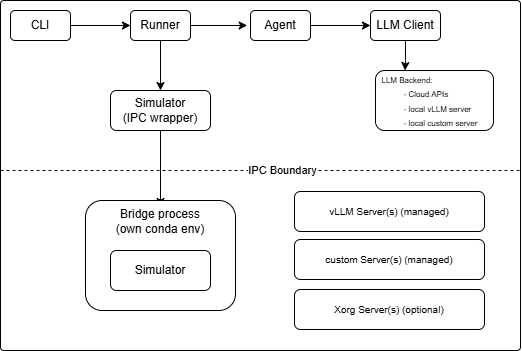
\includegraphics[width=0.7\textwidth]{fig/easi_arch.png}
\caption{High-level architecture of the EASI embodied evaluation library. The subprocess boundary separates the host process (Python 3.10+) from simulator bridge processes that may run different Python versions. Communication uses atomic JSON file I/O. See Appendix~\ref{sec:appendix_architecture} for detailed process flow.}
\label{fig:architecture}
\end{figure}

\subsection{Unified Multi-Simulator Evaluation}

The core architectural insight is \textbf{subprocess isolation}. Each simulator runs in its own conda environment, potentially with a different Python version. AI2-THOR v2.1 requires Python 3.8, Habitat-Sim requires Python 3.9, while the host runs Python 3.10+. A bridge script inside each simulator's environment communicates with the parent process through filesystem-based IPC, using atomic JSON file reads and writes in a temporary directory. This avoids the complexity of socket-based communication while maintaining reliability across Python version boundaries. The IPC protocol uses three files (\texttt{status.json}, \texttt{command.json}, and \texttt{response.json}) with atomic writes via rename to prevent partial reads (see Appendix~\ref{sec:appendix_ipc}).

On top of this isolation layer, the library provides a unified interface. A single CLI command (\texttt{easi start}) with a task name, agent type, backend, and model works identically across all benchmarks. Tasks are auto-discovered via YAML configuration files; simulators are registered through manifest files. Adding a new benchmark requires only a task directory with a YAML config and a Python class, with no modification to any central registry. For benchmarks with multiple evaluation splits (EmbodiedBench has 19 splits across four domains), YAML template inheritance keeps configuration DRY, where split-specific configs extend a shared base via \texttt{extends:~\_base.yaml}, varying only the dataset subset, episode filter, or action space.

\subsection{Standardised Agent-Environment Interface}

A key challenge in embodied evaluation is that different benchmarks require different prompt formats, action spaces, and feedback mechanisms. The library addresses this through a \textbf{PromptBuilder} protocol that standardises the agent-environment interface while remaining customisable per benchmark.

The standard prompt format uses a two-message structure as shown in Figure~\ref{fig:prompt_structure}. The system prompt follows a fixed section order (Role and Environment, Available Actions, Strategy, Guidelines, and Response Format), providing the LLM with a consistent frame of reference regardless of which benchmark is running. The user message assembles per-step dynamic content, including the current camera image, task instruction, environment feedback (e.g., geodesic distance to goal), and a truncated action history showing previous actions and their outcomes. A complete prompt example for a navigation episode is provided in Appendix~\ref{sec:appendix_prompt}.

\begin{figure}[htbp]
\centering
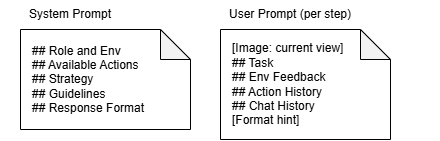
\includegraphics[width=0.7\textwidth]{fig/prompt.png}
\caption{Standardised prompt structure. The system prompt is static per benchmark; the user message is assembled fresh each step with current observations and history.}
\label{fig:prompt_structure}
\end{figure}

The LLM responds in a standardised 4-field JSON format: a visual state description, reasoning and reflection, a language plan, and an executable plan containing a list of actions. This structured format enables \textit{multi-action buffering}. When the LLM generates a plan with multiple actions, the agent executes them one at a time without re-prompting the LLM until an action fails or the buffer is exhausted, substantially reducing API calls.

\subsection{Scalable Parallel Evaluation}

Embodied evaluation is time-intensive. A single EB-Alfred episode may involve 50+ LLM calls with image inputs, and a full benchmark can take hours to complete sequentially. To make large-scale evaluation practical, the library supports \textit{thread-pool parallelism} where each worker gets its own simulator process, agent instance, and LLM client. Workers pull episodes from a shared thread-safe queue, enabling automatic load balancing.

For local inference using vLLM, the library manages the full server lifecycle. A \texttt{MultiServerManager} spawns multiple vLLM instances across designated GPUs using a two-phase startup (spawn all processes, then concurrent health checks), distributes workers across instances via round-robin URL assignment, and tears down servers on completion. GPU allocation is explicitly partitioned into separate pools for LLM inference and simulator rendering, preventing resource contention. A render platform abstraction handles the diverse display requirements of different simulators, supporting six backends (native X11, virtual framebuffer, EGL headless, managed Xorg, and others) with per-worker GPU binding. See Appendix~\ref{sec:appendix_parallel} for detailed worker lifecycle and resource management.

\subsection{Reproducibility and Analysis}

Long-running evaluations need robust support for interruption and resumption. The library saves a configuration file with all CLI options at run start, and each completed episode writes its metrics and step-by-step trajectory (including observation images) to a structured output directory. A resume flag restarts from the last completed episode, re-aggregating results across both completed and new episodes.

An episode filtering syntax supports index ranges, specific episode IDs, and mixed specifications, enabling targeted re-evaluation of particular episodes without rerunning the full benchmark.

\section{The Breadth of Embodied Evaluation}

Before implementing the library's architecture, I had spent several weeks verifying each of the EmbodiedBench~\cite{yang2025embodiedbenchcomprehensivebenchmarkingmultimodal} environments (Alfred, Navigation, Habitat, and Manipulation), setting up their respective simulators on the server and confirming that episodes could be loaded, reset, and stepped through correctly. This groundwork informed the library's design and ensured that the abstractions I chose would accommodate the real diversity of simulator interfaces.

The library now integrates ten embodied benchmarks spanning five simulators and a wide range of capabilities.

EmbodiedBench's four domains alone cover 19 evaluation splits. \textbf{EB-Alfred} (AI2-THOR v2.1) tests household task completion across six capability dimensions, namely base, spatial, visual, commonsense, complex instruction following, and long-horizon planning. A ``complex'' episode might require the agent to execute 20+ sequential actions (``heat the potato, then put it on the counter, then pick up the knife\ldots''), while a ``spatial'' episode tests whether the agent can locate objects based on spatial descriptions. \textbf{EB-Navigation} (AI2-THOR v5.0) evaluates indoor point-goal navigation with five splits. \textbf{EB-Habitat} (Habitat-Sim) tests scene understanding combined with navigation across four splits. \textbf{EB-Manipulation} (CoppeliaSim) evaluates robotic manipulation, specifically precise 3D gripper positioning using discrete action coordinates.

Beyond EmbodiedBench, the library integrates \textbf{HAZARD}~\cite{zhou2024hazardchallengeembodieddecision} (ThreeDWorld), which presents a qualitatively different challenge. The agent must infer \textit{implicit} goals under emergency conditions. During a fire scenario, the agent is not told ``evacuate the laptop'' but instead must reason that valuable objects should be rescued and identify which objects are valuable, all while navigating a dynamically changing environment. This tests what I term \textit{situational goal reasoning}, a capability not captured by any static benchmark.

\textbf{ManipulaTHOR}~\cite{ehsani2021manipulathorframeworkvisualobject} tests arm-based point navigation in AI2-THOR, and \textbf{AI2-THOR Rearrangement 2023}~\cite{RoomR} evaluates an agent's ability to restore objects to their original positions across five evaluation splits. The \textbf{VLN-CE}~\cite{krantz2020navgraphvisionandlanguagenavigationcontinuous} benchmarks (R2R and RxR) bring vision-and-language navigation into continuous environments using Habitat-Sim, requiring agents to translate free-form natural language instructions (``Walk past the dining table, turn left at the hallway, stop at the second door on your right'') into continuous movement. The RxR variant includes Hindi and Telugu instructions, enabling multilingual embodied evaluation. \textbf{LHPR-VLN}~\cite{song2025longhorizonvisionlanguagenavigationplatform} extends this with multi-subtask navigation requiring hierarchical planning.

\section{The LLM-Driven Agent}

To drive evaluation across these diverse benchmarks, the library implements an LLM-driven agent that follows a perceive-reason-act loop. At each step, the agent receives an egocentric camera image and environment feedback from the simulator. It maintains an \textbf{agent memory} that tracks the full interaction history, including previous observations, actions taken, environment feedback received, and the LLM's own prior responses, providing the context needed for coherent multi-step behaviour. The PromptBuilder (Section~\ref{sec:embodied}) assembles this memory into a structured prompt, which is sent to the LLM for reasoning. The LLM returns a structured response containing its visual description of the scene, reasoning about the current situation, a natural language plan, and one or more proposed actions. The agent validates each action against the task's action space and executes them sequentially.

Two mechanisms make this loop practical at scale. First, \textbf{multi-action buffering}. When the LLM generates a plan with multiple actions, the agent executes them one at a time without re-prompting the LLM until an action fails or the buffer is exhausted, substantially reducing API calls. Second, \textbf{feedback-driven replanning}. When an action fails, the failure is recorded in the action history, the action buffer is cleared, and the agent re-prompts the LLM with the updated context on the next step. This enables error recovery without explicit failure-handling logic. The LLM reasons about what went wrong based on the feedback history and adjusts its plan accordingly.

The agent interface is pluggable as the current implementation uses an LLM for reasoning, but the library also includes a dummy agent (random action selection) for testing, and the protocol is designed so that alternative agent architectures, such as those incorporating explicit spatial maps or hierarchical planners, can be substituted without modifying the evaluation pipeline.

\section{What Embodied Evaluation Adds to the Picture}

The capability dimensions tested by embodied benchmarks partially overlap with the EASI static taxonomy but extend it in important ways. Static benchmarks test whether a model can answer \textit{``which object is to the left of the chair?''}, while embodied benchmarks test whether an agent can \textit{navigate to} the left of the chair, pick up the object there, and carry it to another room. This requires not just spatial perception (SR) and perspective-taking (PT), but also the following.

\begin{itemize}
    \item \textbf{Long-horizon planning}: Decomposing complex goals into executable action sequences, maintaining a mental model of progress, and deciding when to replan.
    \item \textbf{Situational goal reasoning}: Inferring what to do when the goal is not explicitly stated (HAZARD scenarios).
    \item \textbf{Grounded language understanding}: Translating natural language navigation instructions into continuous movement through 3D space (VLN-CE).
    \item \textbf{Error recovery}: Detecting when an action has failed (a gripper didn't close, a navigation step was blocked) and adapting the plan accordingly.
\end{itemize}

The preliminary finding from~\cite{cai2025scalingspatialintelligencemultimodal}, that SenseNova-SI improved EmbodiedBench manipulation performance without fine-tuning, is encouraging. The EASI embodied library now makes it possible to test this transfer systematically across all ten benchmarks and multiple model families, providing a much richer picture of whether and how static spatial intelligence translates to embodied competence.

\section{Preliminary Experiment: EASI-Mini}

To provide an initial data point on whether static spatial intelligence gains transfer to embodied settings, I designed and ran a compact cross-benchmark evaluation called EASI-Mini. The benchmark samples 74 episodes across six capability dimensions from the library's integrated benchmarks, enabling a structured comparison without the cost of running all ten benchmarks at full scale.

The benchmark is designed such that each capability dimension draws episodes from one or more source benchmarks, as summarised in Table~\ref{tab:easimini_design}. Episodes are sampled deterministically (seed 42) for reproducibility. Success is normalized across benchmarks, using \texttt{task\_success} for EmbodiedBench and \texttt{success} (within 3m of goal) for VLN-CE.

\begin{table}[htbp]
\centering
\caption{EASI-Mini benchmark design: capability dimensions and episode sources.}
\label{tab:easimini_design}
\renewcommand{\arraystretch}{1.1}
\small
\begin{tabular}{lp{4.5cm}r}
\toprule
\textbf{Capability} & \textbf{Sources} & \textbf{Eps} \\
\midrule
Spatial Reasoning & EB-Alfred, EB-Habitat, EB-Manipulation & 9 \\
Common Sense & EB-Alfred, EB-Navigation, EB-Habitat, EB-Manipulation & 12 \\
Complex Instruction & EB-Alfred, EB-Navigation, EB-Habitat, EB-Manipulation & 12 \\
Long-Horizon Planning & EB-Alfred, EB-Habitat, LHPR-VLN & 14 \\
Visual Grounding & EB-Alfred, EB-Navigation, EB-Habitat, EB-Manipulation & 12 \\
Continuous Navigation & VLN-CE R2R (val unseen) & 15 \\
\midrule
\textbf{Total} & & \textbf{74} \\
\bottomrule
\end{tabular}
\end{table}

For model evaluation, four models were selected to span the proprietary--open-source axis and to test the effect of spatial data scaling. \textbf{GPT-5.2} serves as a proprietary baseline with strong general vision capabilities. \textbf{Qwen3-8B-Instruct} is a competitive open-source model from the static evaluation (Chapter~\ref{sec:diagnosis}). \textbf{InternVL3-8B} provides the base model before spatial data scaling, while \textbf{SenseNova-SI InternVL3-8B} is the same model after SFT on SenseNova-SI-8M spatial data as described in Chapter~\ref{sec:treatment}.

The InternVL3-8B vs.\ SenseNova-SI InternVL3-8B comparison directly tests the central question of whether the dramatic improvement on static spatial benchmarks (e.g., 41.5\% $\to$ 85.6\% on MindCube) translates into better embodied performance.

\begin{table}[htbp]
\centering
\caption{EASI-Mini results: success rate (\%) by capability dimension.}
\label{tab:easimini_capability}
\renewcommand{\arraystretch}{1.1}
\begin{tabular}{lcccc}
\toprule
\textbf{Capability} & \textbf{GPT-5.2} & \textbf{Qwen3-8B} & \textbf{InternVL3-8B} & \textbf{SN-SI InternVL3-8B} \\
\midrule
Spatial Reasoning & 33.3 & 11.1 & 11.1 & 0.0 \\
Common Sense & 41.7 & 16.7 & 8.3 & 0.0 \\
Complex Instruction & 33.3 & 16.7 & 16.7 & 8.3 \\
Long-Horizon Planning & 28.6 & 0.0 & 0.0 & 0.0 \\
Visual Grounding & 58.3 & 25.0 & 16.7 & 0.0 \\
Continuous Navigation & 33.3 & 0.0 & 6.7 & 0.0 \\
\midrule
\textbf{Overall} & \textbf{37.8} & \textbf{10.8} & \textbf{9.5} & \textbf{1.4} \\
\bottomrule
\end{tabular}
\end{table}

\begin{table}[htbp]
\centering
\caption{EASI-Mini results: success rate (\%) by source benchmark.}
\label{tab:easimini_benchmark}
\renewcommand{\arraystretch}{1.1}
\begin{tabular}{lcccc}
\toprule
\textbf{Benchmark} & \textbf{GPT-5.2} & \textbf{Qwen3-8B} & \textbf{InternVL3-8B} & \textbf{SN-SI InternVL3-8B} \\
\midrule
EB-Alfred & 66.7 & 13.3 & 0.0 & 0.0 \\
EB-Navigation & 66.7 & 22.2 & 22.2 & 11.1 \\
EB-Habitat & 6.7 & 0.0 & 0.0 & 0.0 \\
EB-Manipulation & 41.7 & 33.3 & 33.3 & 0.0 \\
VLN-CE R2R & 33.3 & 0.0 & 6.7 & 0.0 \\
LHPR-VLN & 12.5 & 0.0 & 0.0 & 0.0 \\
\bottomrule
\end{tabular}
\end{table}


\textbf{Analysis.} The results reveal a clear model capability hierarchy. GPT-5.2 (37.8\% overall SR) substantially outperforms all open-source models, followed by Qwen3-8B (10.8\%), InternVL3-8B (9.5\%), and SenseNova-SI InternVL3-8B (1.4\%). Several patterns stand out.

\textbf{Spatial SFT degrades instruction following.} The central question of this experiment was whether SenseNova-SI's dramatic gains on static spatial benchmarks (e.g., 41.5\% $\to$ 85.6\% on MindCube) would translate into better embodied performance. SenseNova-SI InternVL3-8B (1.4\% SR) actually underperforms the base InternVL3-8B (9.5\% SR) across nearly all capability dimensions and benchmarks. However, this does not necessarily mean spatial data scaling is ineffective for embodied tasks. Analysis of the failure modes reveals that the dominant cause of failure is the model's inability to generate well-formed JSON action outputs, leading to parse errors and zero-step episodes. The spatial SFT appears to have degraded the model's instruction-following and structured output capabilities rather than its spatial reasoning per se. Several open-source models, particularly on EB-Manipulation and EB-Habitat, completed episodes with zero steps taken for this reason. Future work on spatial data curation should consider preserving instruction-following ability during SFT, perhaps through mixed training with general-purpose data.

\textbf{Proprietary models hold a decisive advantage.} GPT-5.2 leads across every capability dimension and every benchmark. The gap is particularly large on EB-Alfred (66.7\% vs 13.3\% for the next best) and EB-Navigation (66.7\% vs 22.2\%), both of which require multi-step planning and structured action output. This suggests that embodied tasks benefit from capabilities beyond spatial perception, including instruction following, action grounding, and error recovery, where larger proprietary models excel.

\textbf{Long-horizon planning is the weakest capability.} Across all models, long-horizon planning and continuous navigation yield the lowest success rates, while visual grounding is consistently the strongest (58.3\% for GPT-5.2, 25.0\% for Qwen3-8B). One contributing factor may be the evaluation setup. The current agent uses only action history (previous actions and their outcomes) but not full chat history (the model's own prior reasoning). Without access to its earlier reasoning traces, the model cannot build on previous plans or maintain coherent long-term strategies, which disproportionately affects tasks requiring many sequential steps.

This experiment is preliminary. Each capability dimension samples only 3 to 5 episodes per benchmark. The small sample sizes limit statistical robustness, and the results should not be treated as definitive assessments of model capability. Nevertheless, EASI-Mini demonstrates the library's ability to produce structured, cross-benchmark comparisons with a single evaluation script, and provides an initial signal on the static-to-embodied transfer question.

\chapter{Discussion}
\label{sec:discussion}

\section{The Arc of the Work}

Looking back, the three phases of this research form a natural scientific progression. The holistic evaluation (Phase 1) provided the diagnosis, revealing that spatial intelligence is a specific, measurable weakness of current models, worst in perspective-taking and metric measurement, present even in frontier proprietary models, and not reducible to general model scale. The data scaling work (Phase 2) provided a treatment, demonstrating that targeted, taxonomy-guided data curation can produce dramatic improvements, with open-source models matching or exceeding proprietary ones on several challenging subtasks. The embodied evaluation library (Phase 3) provides the infrastructure for the next question, namely whether the treatment works in the real world.

This arc also reflects a progression in my own contributions. In the first phase, I built the evaluation infrastructure that made holistic comparison possible, integrating nine benchmarks and two models into a unified framework, fixing inference bugs that would have corrupted results. In the second phase, this infrastructure was reused to validate the SenseNova-SI models, with the benchmarks and model integrations I had built serving directly as the evaluation backbone and baselines. In the third phase, I worked independently to design and implement an entirely new evaluation toolkit, drawing on the insights from the first two phases to frame embodied evaluation as a natural extension of spatial intelligence research.

\section{Reflections on Evaluation-Driven Research}

A recurring theme is that evaluation infrastructure is not merely a support function but rather shapes the research questions that can be asked. The unified lmms-eval integrations made the holistic comparison in~\cite{cai2025holisticevaluationmultimodalllms} possible; without them, the study would have been a collection of disconnected benchmark scores rather than a coherent capability analysis. The EASI taxonomy, in turn, made the data gap analysis in~\cite{cai2025scalingspatialintelligencemultimodal} actionable. By mapping every benchmark subtask to a capability dimension, the team could identify precisely where training data was lacking (perspective-taking) and scale accordingly.

The embodied evaluation library continues this pattern. By unifying ten benchmarks under a single CLI, it becomes feasible to ask questions like ``does improving MindCube performance predict better EB-Manipulation scores?'' or ``which static capability is most predictive of VLN-CE success?'' These are questions that would be impractical if each benchmark required its own evaluation pipeline.

\section{Limitations and Future Directions}

Several important limitations and open questions remain.

\textbf{Cost of embodied evaluation.} Each embodied episode requires multiple simulator steps and LLM calls, making evaluation orders of magnitude more expensive than static benchmarks. A single EB-Alfred episode may involve 50+ LLM calls with image inputs. Efficient evaluation strategies (episode sampling, proxy metrics, early stopping) will be important for making embodied evaluation routine rather than occasional.

\textbf{EASI-Mini is preliminary.} The EASI-Mini experiment samples only 3 to 5 episodes per benchmark per capability dimension, totalling 74 episodes. At this scale, a single lucky or unlucky episode can swing a benchmark's success rate by 33 percentage points. The results provide directional signals rather than statistically robust estimates. A comprehensive transfer study across all ten embodied benchmarks at full scale, with multiple model families and varying amounts of spatial training data, remains future work.

\textbf{Confounding factors in embodied evaluation.} The EASI-Mini results conflate spatial intelligence with other capabilities such as instruction following, structured output generation, and error recovery. The zero-step failures observed for several open-source models on EB-Manipulation and EB-Habitat suggest that format compliance, rather than spatial reasoning, was the binding constraint. Disentangling these factors would require controlled experiments that isolate spatial reasoning from action grounding.

\textbf{Agent architecture.} The ReAct agent is a reasonable baseline but far from the ceiling. More sophisticated architectures incorporating explicit spatial maps, hierarchical planning, or learned exploration strategies could better leverage spatial intelligence. The library's pluggable agent interface is designed to support this exploration.

\textbf{The CoT puzzle.} The finding that text-based chain-of-thought does not reliably improve spatial reasoning~\cite{cai2025scalingspatialintelligencemultimodal} is both surprising and important. It suggests that spatial reasoning may require fundamentally different mechanisms, perhaps visual or geometric chain-of-thought, or internal 3D representations, rather than the linguistic decomposition that works well for mathematical and logical reasoning.

\textbf{Multilingual embodied evaluation.} The VLN-CE RxR benchmark includes Hindi and Telugu instructions alongside English, enabling multilingual embodied evaluation, an area that remains largely unexplored.

\chapter{Conclusion}
\label{sec:conclusion}

This report has traced a path from measuring spatial intelligence through improving it to evaluating whether improvements transfer to embodied settings. Along the way, I contributed evaluation infrastructure (nine benchmark integrations, two model integrations, and numerous bug fixes in lmms-eval) that enabled the holistic spatial intelligence evaluation reported in~\cite{cai2025holisticevaluationmultimodalllms} and the model validation in~\cite{cai2025scalingspatialintelligencemultimodal}. I then independently designed and built the EASI embodied evaluation library, a unified toolkit integrating ten embodied benchmarks across five simulators with LLM-powered agents, subprocess isolation for heterogeneous Python environments, and a comprehensive evaluation pipeline with parallel execution, episode filtering, resume support, and trajectory analysis. A preliminary cross-benchmark experiment (EASI-Mini) provided initial data on whether static spatial gains transfer to embodied tasks.

The overarching finding of this research is that spatial intelligence is both more important and more tractable than previously assumed. The gap between models and humans is large but not immutable, and targeted data scaling produces dramatic improvements. The EASI-Mini experiment offers a first look at whether these improvements extend from static benchmarks to embodied competence, and the library provides the infrastructure for the comprehensive studies that will follow.


\printbibliography

\appendix
\chapter{EASI Library Architecture Deep-Dive}
\label{sec:appendix_architecture}

\section{Process Flow}
\label{sec:appendix_process}

Figure~\ref{fig:process_flow} shows the full lifecycle of an \texttt{easi start} invocation, from CLI parsing through episode execution to final cleanup. Component interactions proceed top-to-bottom; the subprocess boundary separates the host process from simulator bridge processes.


\begin{figure}[htbp]
\centering
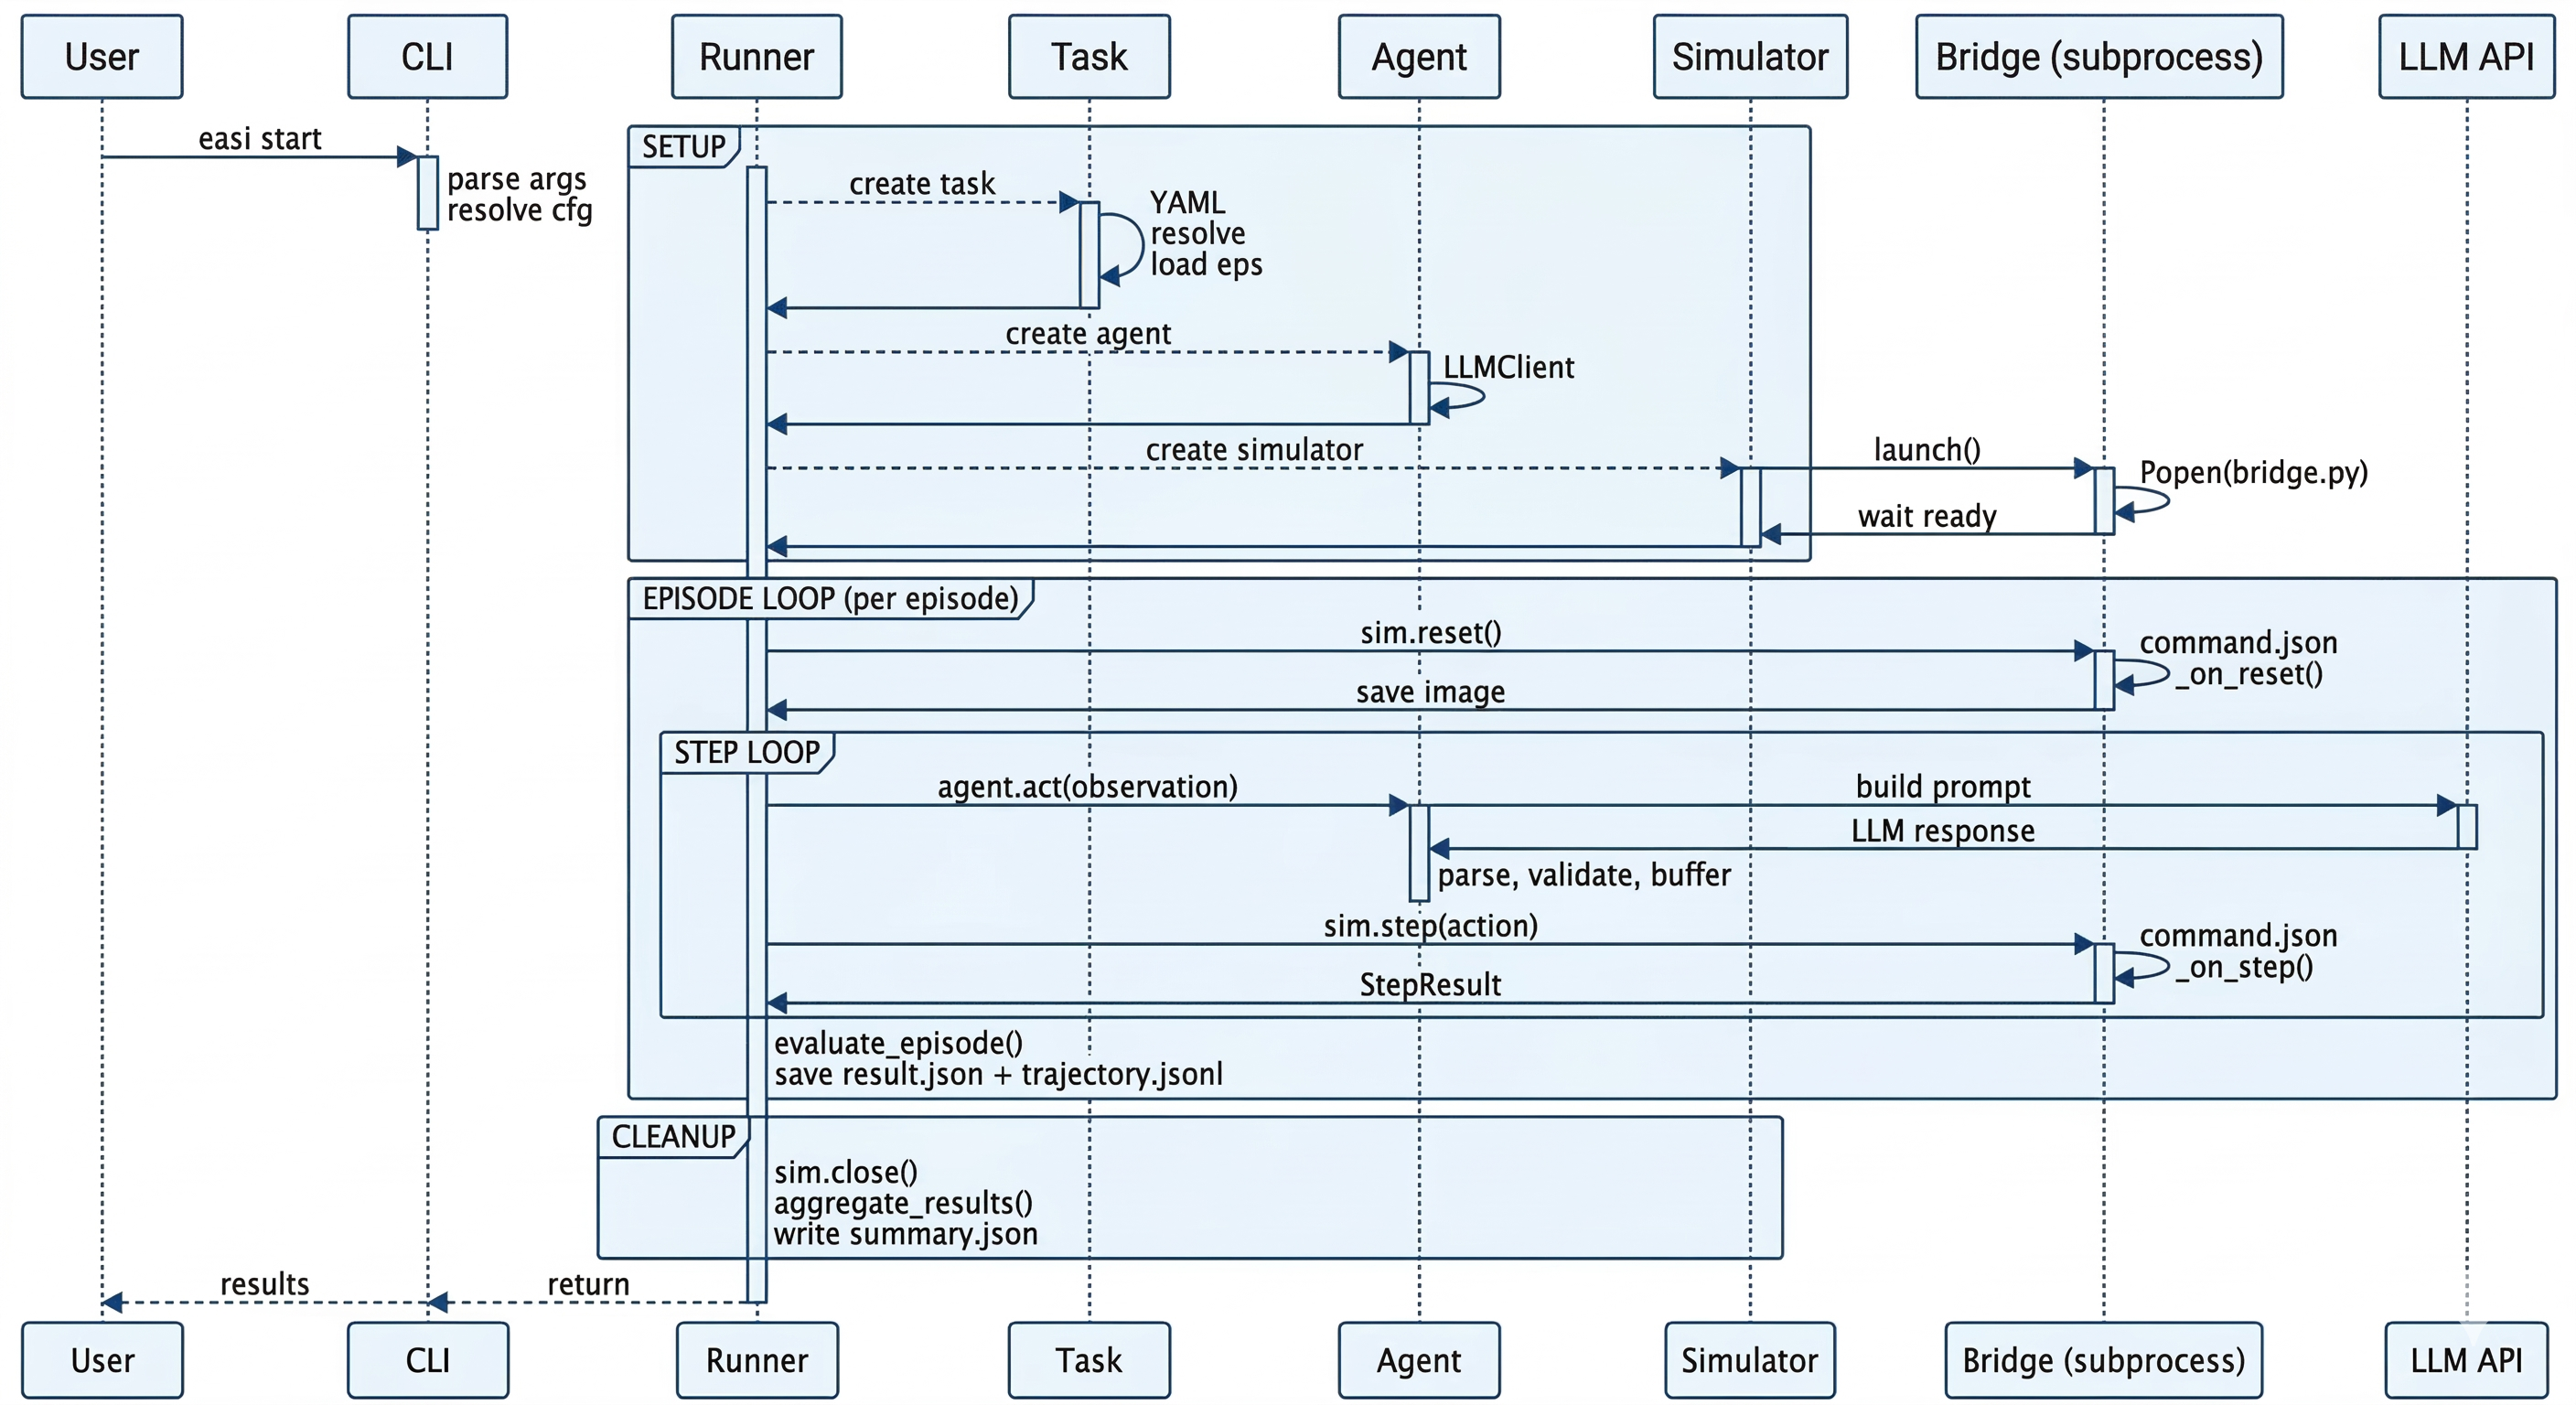
\includegraphics[width=\textwidth]{fig/process_flow.png}
\caption{Sequence diagram showing the full lifecycle of an \texttt{easi start} invocation.}
\label{fig:process_flow}
\end{figure}

\section{IPC Protocol}
\label{sec:appendix_ipc}

Communication between the host process and each simulator bridge uses three JSON files in a temporary workspace directory:

\begin{lstlisting}[basicstyle=\ttfamily\small, numbers=none, backgroundcolor=\color{white}, frame=single]
/tmp/easi_XXXXXXXX/
  status.json       <- bridge writes on startup: {"ready": true}
  command.json      <- parent writes, bridge reads
  response.json     <- bridge writes, parent reads
\end{lstlisting}

All writes use an \textbf{atomic rename} pattern (\texttt{file.tmp} $\to$ \texttt{file.json}) to prevent partial reads. The parent polls \texttt{response.json} with a configurable interval (default 0.1s) and timeout, checking subprocess liveness on each poll. The supported command types are summarised in Table~\ref{tab:ipc_commands}.

\begin{table}[htbp]
\centering
\caption{IPC command types between the parent process and simulator bridge.}
\label{tab:ipc_commands}
\small
\renewcommand{\arraystretch}{1.1}
\begin{tabular}{llll}
\toprule
\textbf{Type} & \textbf{Parent Sends} & \textbf{Bridge Does} & \textbf{Bridge Returns} \\
\midrule
\texttt{reset} & episode\_id, config & Create/reset env & observation, reward, done \\
\texttt{step} & action\_name, params & Execute action & observation, reward, done \\
\texttt{close} & type: ``close'' & Cleanup, exit & status: ``ok'' \\
\bottomrule
\end{tabular}
\end{table}

\begin{table}[htbp]
\centering
\caption{EASI library component map (30+ modules organised by architectural layer).}
\label{tab:component_map}
\small
\renewcommand{\arraystretch}{1.1}
\begin{tabular}{lp{3.5cm}p{4cm}}
\toprule
\textbf{Layer} & \textbf{Components} & \textbf{Role} \\
\midrule
CLI \& Orchestration & \texttt{cli.py}, Runners, EpisodeFilter, Metrics & Parse args, manage episode loop, aggregate \\
Tasks & TaskRegistry, yaml\_utils, Dataset, BaseTask & Auto-discover, YAML inheritance, load datasets \\
Agents & ReActAgent, AgentMemory, PromptBuilder & LLM decisions, state tracking, prompt assembly \\
LLM & LLMClient, ServerManager, DummyServer & Unified LLM interface, vLLM lifecycle \\
Simulators & SimulatorRegistry, SubprocessRunner, BaseBridge & Auto-discover, IPC, process lifecycle \\
Communication & filesystem.py, schemas.py & Atomic JSON I/O, schemas \\
Rendering & RenderPlatform, XorgManager, Adapters & Display backend, Xorg servers, adjustments \\
Analysis & TrajectoryVideo, ProgressBar & Post-hoc video, progress display \\
\bottomrule
\end{tabular}
\end{table}

\section{Parallel Execution and Resource Management}
\label{sec:appendix_parallel}

The \texttt{ParallelRunner} extends the sequential runner with thread-pool concurrency. Each worker is fully isolated with its own simulator process, agent instance, and LLM client.

\begin{figure}[htbp]
\centering
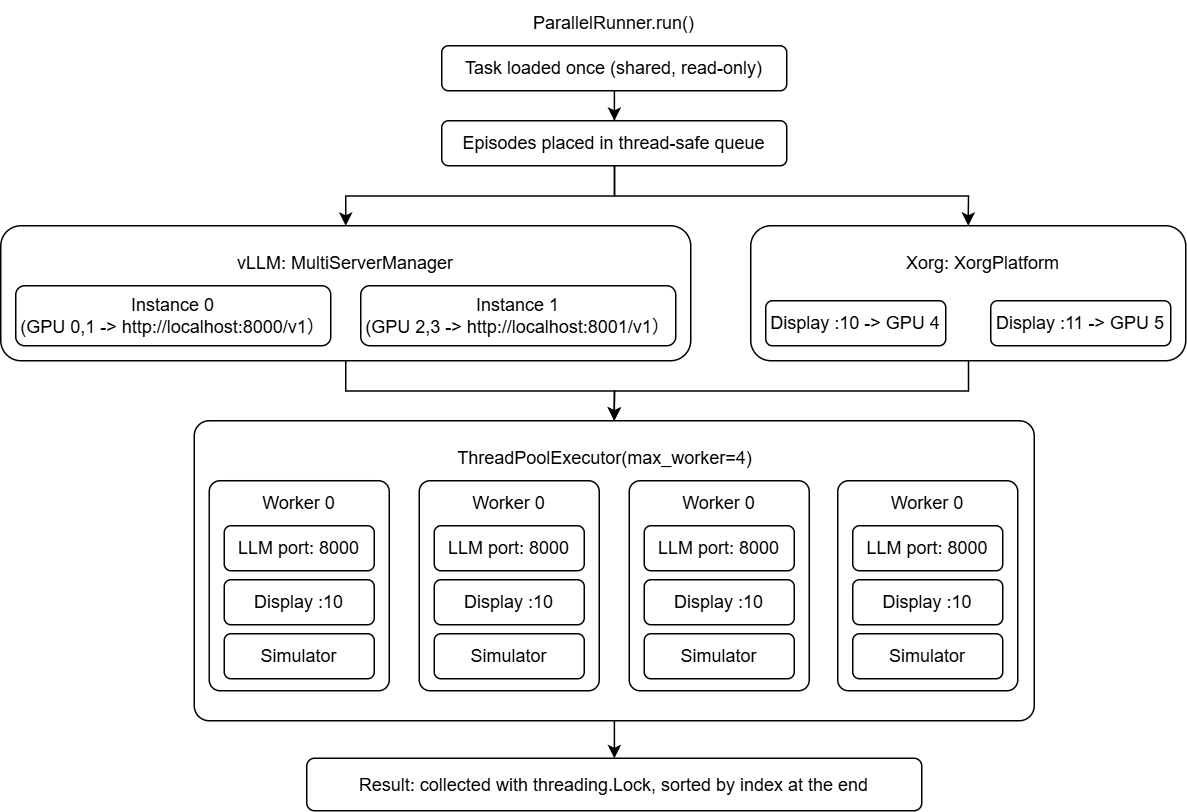
\includegraphics[width=\textwidth]{fig/parallel_flow.png}
\caption{ParallelRunner execution flow with thread-pool concurrency, multi-instance vLLM, and Xorg display management.}
\label{fig:parallel_flow}
\end{figure}

Resource assignment uses round-robin allocation:
\begin{itemize}
    \item LLM URLs: \texttt{base\_urls[worker\_id \% len(base\_urls)]} distributes workers evenly across vLLM instances
    \item GPU/display binding: \texttt{platform.for\_worker(worker\_id)} cycles through available render instances
    \item Thread-safe results: \texttt{threading.Lock} guards the shared results list
\end{itemize}

\begin{table}[htbp]
\centering
\caption{Render platform hierarchy and use cases.}
\label{tab:render_platforms}
\small
\renewcommand{\arraystretch}{1.1}
\begin{tabular}{llll}
\toprule
\textbf{Platform} & \textbf{Display} & \textbf{GPU Binding} & \textbf{Use Case} \\
\midrule
\texttt{auto} & Detect; fallback xvfb & Manual & Default \\
\texttt{native} & Existing \texttt{\$DISPLAY} & Manual & Desktop with X \\
\texttt{xvfb} & Virtual framebuffer & Manual & Headless (CPU) \\
\texttt{egl} & None (headless) & CUDA\_VISIBLE & GPU headless \\
\texttt{headless} & None & Manual & Native headless \\
\texttt{xorg} & \texttt{:N} per GPU & Auto-managed & GPU X11 \\
\bottomrule
\end{tabular}
\end{table}


\chapter{Prompt Format and Full Example}
\label{sec:appendix_prompt}

\section{Prompt Format Specification}

The EASI standard prompt format defines how the agent communicates with any LLM backend. It applies to all benchmarks that do not have a published prompt format (EmbodiedBench benchmarks retain their original formats for reproducibility). The system prompt follows a fixed section order as shown in Table~\ref{tab:prompt_sections}.

\begin{table}[htbp]
\centering
\caption{System prompt sections and their purposes.}
\label{tab:prompt_sections}
\small
\renewcommand{\arraystretch}{1.1}
\begin{tabular}{lcp{5cm}}
\toprule
\textbf{Section} & \textbf{Req.} & \textbf{Purpose} \\
\midrule
Role and Environment & Yes & Agent identity and environment \\
Observation Description & No & Non-visual feedback explanation \\
Available Actions & Yes & Action names, descriptions, params \\
Strategy & No & Benchmark-specific tactical advice \\
Guidelines & Yes & Universal rules \\
Response Format & Yes & The 4-field JSON schema \\
\bottomrule
\end{tabular}
\end{table}

The response follows a 4-field JSON schema as shown below.
\begin{lstlisting}[language=Java, basicstyle=\ttfamily\small, numbers=none]
{
    "visual_state_description": "Describe what you see",
    "reasoning_and_reflection": "Reason about situation",
    "language_plan": "Describe next plan",
    "executable_plan": [
        {"action": "move_forward"},
        {"action": "turn_left"}
    ]
}
\end{lstlisting}

The user message is assembled per step in the following order.
\begin{lstlisting}[basicstyle=\ttfamily\small, numbers=none, backgroundcolor=\color{white}, frame=single]
[Image(s)]                    <- base64 encoded
[Text content:]
  ## Task                     <- instruction
  ## Environment Feedback     <- current-step feedback
  ## Action History (last N)  <- compact action + outcome log
  ## Chat History (last N)    <- previous LLM responses
  [Response format reminder]  <- brief JSON format hint
\end{lstlisting}

\section{Complete Prompt Example: Navigation Episode}

The following shows the exact prompt sent to the LLM during step 5 of a VLN-CE navigation episode.

The system prompt for this episode is shown below.

\begin{lstlisting}[basicstyle=\ttfamily\small, numbers=none, backgroundcolor=\color{backcolour}]
## Role and Environment
You are a robot navigating in a 3D indoor environment.
You observe the environment through a front-facing camera
and must follow natural language instructions to navigate
to a goal location.

## Observation Description
- **Distance to goal**: Geodesic distance in meters to
  the goal. Decreases as you approach the destination.

## Available Actions
- move_forward: Move forward by 0.25 meters
- turn_left: Turn left by 15 degrees
- turn_right: Turn right by 15 degrees
- stop: Stop and end navigation (use ONLY when you
  believe you have reached the destination)

## Strategy
1. Carefully read the navigation instruction
2. Observe your surroundings in the image
3. Follow the instruction step by step
4. Use stop ONLY when confident you have reached
   the described destination

## Guidelines
1. Always output at least one action.
2. Only use actions from the Available Actions list.
3. If previous actions failed, try a different approach.
4. Do not repeatedly execute the same action sequence.
5. Keep your plan efficient and concise.

## Response Format
Output a JSON object with exactly these 4 fields:
{
    "visual_state_description": "...",
    "reasoning_and_reflection": "...",
    "language_plan": "...",
    "executable_plan": [{"action": "<action_name>"}]
}
\end{lstlisting}

The user message at step 5 is as follows.


\begin{lstlisting}[basicstyle=\ttfamily\small, numbers=none, backgroundcolor=\color{backcolour}]
[Image: base64 encoded current view]

## Task
Walk down the hallway and turn right into the bedroom.

## Environment Feedback
Distance to goal: 5.3m

## Action History (last 5 steps)
Step 0: move_forward -> Distance to goal: 8.2m
Step 1: move_forward -> Distance to goal: 7.9m
Step 2: move_forward -> Distance to goal: 7.6m
Step 3: turn_right -> Distance to goal: 7.6m
Step 4: move_forward -> Distance to goal: 7.3m

Respond with the JSON format specified above.
\end{lstlisting}


\end{document}
